% Options for packages loaded elsewhere
\PassOptionsToPackage{unicode}{hyperref}
\PassOptionsToPackage{hyphens}{url}
%
\documentclass[
]{article}
\usepackage{lmodern}
\usepackage{amssymb,amsmath}
\usepackage{ifxetex,ifluatex}
\ifnum 0\ifxetex 1\fi\ifluatex 1\fi=0 % if pdftex
  \usepackage[T1]{fontenc}
  \usepackage[utf8]{inputenc}
  \usepackage{textcomp} % provide euro and other symbols
\else % if luatex or xetex
  \usepackage{unicode-math}
  \defaultfontfeatures{Scale=MatchLowercase}
  \defaultfontfeatures[\rmfamily]{Ligatures=TeX,Scale=1}
\fi
% Use upquote if available, for straight quotes in verbatim environments
\IfFileExists{upquote.sty}{\usepackage{upquote}}{}
\IfFileExists{microtype.sty}{% use microtype if available
  \usepackage[]{microtype}
  \UseMicrotypeSet[protrusion]{basicmath} % disable protrusion for tt fonts
}{}
\makeatletter
\@ifundefined{KOMAClassName}{% if non-KOMA class
  \IfFileExists{parskip.sty}{%
    \usepackage{parskip}
  }{% else
    \setlength{\parindent}{0pt}
    \setlength{\parskip}{6pt plus 2pt minus 1pt}}
}{% if KOMA class
  \KOMAoptions{parskip=half}}
\makeatother
\usepackage{xcolor}
\IfFileExists{xurl.sty}{\usepackage{xurl}}{} % add URL line breaks if available
\IfFileExists{bookmark.sty}{\usepackage{bookmark}}{\usepackage{hyperref}}
\hypersetup{
  pdftitle={gtsummary},
  pdfauthor={Daniel D. Sjoberg, Karissa Whiting, Margaret Hannum, Emily C. Zabor, Michael Curry},
  hidelinks,
  pdfcreator={LaTeX via pandoc}}
\urlstyle{same} % disable monospaced font for URLs
\usepackage[margin=1in]{geometry}
\usepackage{color}
\usepackage{fancyvrb}
\newcommand{\VerbBar}{|}
\newcommand{\VERB}{\Verb[commandchars=\\\{\}]}
\DefineVerbatimEnvironment{Highlighting}{Verbatim}{commandchars=\\\{\}}
% Add ',fontsize=\small' for more characters per line
\usepackage{framed}
\definecolor{shadecolor}{RGB}{248,248,248}
\newenvironment{Shaded}{\begin{snugshade}}{\end{snugshade}}
\newcommand{\AlertTok}[1]{\textcolor[rgb]{0.94,0.16,0.16}{#1}}
\newcommand{\AnnotationTok}[1]{\textcolor[rgb]{0.56,0.35,0.01}{\textbf{\textit{#1}}}}
\newcommand{\AttributeTok}[1]{\textcolor[rgb]{0.77,0.63,0.00}{#1}}
\newcommand{\BaseNTok}[1]{\textcolor[rgb]{0.00,0.00,0.81}{#1}}
\newcommand{\BuiltInTok}[1]{#1}
\newcommand{\CharTok}[1]{\textcolor[rgb]{0.31,0.60,0.02}{#1}}
\newcommand{\CommentTok}[1]{\textcolor[rgb]{0.56,0.35,0.01}{\textit{#1}}}
\newcommand{\CommentVarTok}[1]{\textcolor[rgb]{0.56,0.35,0.01}{\textbf{\textit{#1}}}}
\newcommand{\ConstantTok}[1]{\textcolor[rgb]{0.00,0.00,0.00}{#1}}
\newcommand{\ControlFlowTok}[1]{\textcolor[rgb]{0.13,0.29,0.53}{\textbf{#1}}}
\newcommand{\DataTypeTok}[1]{\textcolor[rgb]{0.13,0.29,0.53}{#1}}
\newcommand{\DecValTok}[1]{\textcolor[rgb]{0.00,0.00,0.81}{#1}}
\newcommand{\DocumentationTok}[1]{\textcolor[rgb]{0.56,0.35,0.01}{\textbf{\textit{#1}}}}
\newcommand{\ErrorTok}[1]{\textcolor[rgb]{0.64,0.00,0.00}{\textbf{#1}}}
\newcommand{\ExtensionTok}[1]{#1}
\newcommand{\FloatTok}[1]{\textcolor[rgb]{0.00,0.00,0.81}{#1}}
\newcommand{\FunctionTok}[1]{\textcolor[rgb]{0.00,0.00,0.00}{#1}}
\newcommand{\ImportTok}[1]{#1}
\newcommand{\InformationTok}[1]{\textcolor[rgb]{0.56,0.35,0.01}{\textbf{\textit{#1}}}}
\newcommand{\KeywordTok}[1]{\textcolor[rgb]{0.13,0.29,0.53}{\textbf{#1}}}
\newcommand{\NormalTok}[1]{#1}
\newcommand{\OperatorTok}[1]{\textcolor[rgb]{0.81,0.36,0.00}{\textbf{#1}}}
\newcommand{\OtherTok}[1]{\textcolor[rgb]{0.56,0.35,0.01}{#1}}
\newcommand{\PreprocessorTok}[1]{\textcolor[rgb]{0.56,0.35,0.01}{\textit{#1}}}
\newcommand{\RegionMarkerTok}[1]{#1}
\newcommand{\SpecialCharTok}[1]{\textcolor[rgb]{0.00,0.00,0.00}{#1}}
\newcommand{\SpecialStringTok}[1]{\textcolor[rgb]{0.31,0.60,0.02}{#1}}
\newcommand{\StringTok}[1]{\textcolor[rgb]{0.31,0.60,0.02}{#1}}
\newcommand{\VariableTok}[1]{\textcolor[rgb]{0.00,0.00,0.00}{#1}}
\newcommand{\VerbatimStringTok}[1]{\textcolor[rgb]{0.31,0.60,0.02}{#1}}
\newcommand{\WarningTok}[1]{\textcolor[rgb]{0.56,0.35,0.01}{\textbf{\textit{#1}}}}
\usepackage{longtable,booktabs}
% Correct order of tables after \paragraph or \subparagraph
\usepackage{etoolbox}
\makeatletter
\patchcmd\longtable{\par}{\if@noskipsec\mbox{}\fi\par}{}{}
\makeatother
% Allow footnotes in longtable head/foot
\IfFileExists{footnotehyper.sty}{\usepackage{footnotehyper}}{\usepackage{footnote}}
\makesavenoteenv{longtable}
\usepackage{graphicx}
\makeatletter
\def\maxwidth{\ifdim\Gin@nat@width>\linewidth\linewidth\else\Gin@nat@width\fi}
\def\maxheight{\ifdim\Gin@nat@height>\textheight\textheight\else\Gin@nat@height\fi}
\makeatother
% Scale images if necessary, so that they will not overflow the page
% margins by default, and it is still possible to overwrite the defaults
% using explicit options in \includegraphics[width, height, ...]{}
\setkeys{Gin}{width=\maxwidth,height=\maxheight,keepaspectratio}
% Set default figure placement to htbp
\makeatletter
\def\fps@figure{htbp}
\makeatother
\setlength{\emergencystretch}{3em} % prevent overfull lines
\providecommand{\tightlist}{%
  \setlength{\itemsep}{0pt}\setlength{\parskip}{0pt}}
\setcounter{secnumdepth}{-\maxdimen} % remove section numbering

\title{gtsummary}
\author{Daniel D. Sjoberg, Karissa Whiting, Margaret Hannum, Emily C.
Zabor, Michael Curry}
\date{}

\begin{document}
\maketitle

\hypertarget{introduction}{%
\subsection{Introduction}\label{introduction}}

\hypertarget{data-summaries}{%
\subsection{Data Summaries}\label{data-summaries}}

The most common summary needed for research projects are simple
summaries of data sets. To show use of gtsummary functions, we will use
a simulated clinical trial data set containing baseline characteristics
of 200 patients who received Drug A or Drug B as well as the outcome of
tumor response to the treatment. The data set has label attributes
(using the labelled package) for column names.

\begin{longtable}[]{@{}llll@{}}
\caption{Example data frame, \texttt{trial}}\tabularnewline
\toprule
colname & label & class & values\tabularnewline
\midrule
\endfirsthead
\toprule
colname & label & class & values\tabularnewline
\midrule
\endhead
trt & Chemotherapy Treatment & character & \texttt{Drug\ A},
\texttt{Drug\ B}\tabularnewline
age & Age & numeric & \texttt{6}, \texttt{9}, \texttt{10}, \texttt{17} ,
\ldots{}\tabularnewline
marker & Marker Level (ng/mL) & numeric & \texttt{0.003},
\texttt{0.005}, \texttt{0.013}, \texttt{0.015} , \ldots{}\tabularnewline
stage & T Stage & factor & \texttt{T1}, \texttt{T2}, \texttt{T3},
\texttt{T4}\tabularnewline
grade & Grade & factor & \texttt{I}, \texttt{II},
\texttt{III}\tabularnewline
response & Tumor Response & integer & \texttt{0},
\texttt{1}\tabularnewline
death & Patient Died & integer & \texttt{0}, \texttt{1}\tabularnewline
ttdeath & Months to Death/Censor & numeric & \texttt{3.53},
\texttt{5.33}, \texttt{6.32}, \texttt{7.27} , \ldots{}\tabularnewline
\bottomrule
\end{longtable}

\hypertarget{tbl_summary}{%
\subsubsection{\texorpdfstring{\texttt{tbl\_summary()}}{tbl\_summary()}}\label{tbl_summary}}

The \texttt{tbl\_summary()} function can be used to easily create a
basic summary statistic table. This is often the first table of clinical
manuscripts and describes characteristics of the cohort under study. A
simple example is shown below with some basic customizations using the
function's main arguments. Notably, by specifying the ``by'' argument,
you can divide your summary statistic into comparator groups. In this
case, we will split the table by treatment arms.

\begin{Shaded}
\begin{Highlighting}[]
\NormalTok{tbl\_summary\_}\DecValTok{1}\NormalTok{ <{-}}
\StringTok{  }\NormalTok{trial }\OperatorTok{\%>\%}
\StringTok{  }\KeywordTok{select}\NormalTok{(age, grade, response, trt) }\OperatorTok{\%>\%}
\StringTok{  }\KeywordTok{tbl\_summary}\NormalTok{(}\DataTypeTok{by =}\NormalTok{ trt)}
\end{Highlighting}
\end{Shaded}

\begin{figure}[h!]
  \caption{Basic `tbl\_summary()` example}
  \label{fig:summary_basic}
  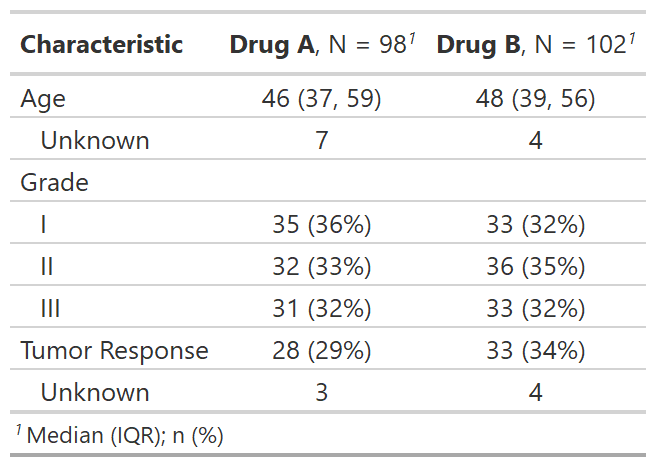
\includegraphics[height=5cm]{tbl_summary_1.png}
  \centering
\end{figure}

\ref{fig:summary_basic} is basic

\hypertarget{tbl_svysummary}{%
\subsubsection{\texorpdfstring{\texttt{tbl\_svysummary()}}{tbl\_svysummary()}}\label{tbl_svysummary}}

\hypertarget{tbl_cross}{%
\subsubsection{\texorpdfstring{\texttt{tbl\_cross()}}{tbl\_cross()}}\label{tbl_cross}}

\hypertarget{tbl_survfit}{%
\subsubsection{\texorpdfstring{\texttt{tbl\_survfit()}}{tbl\_survfit()}}\label{tbl_survfit}}

\hypertarget{customization}{%
\subsubsection{Customization}\label{customization}}

\hypertarget{model-summaries}{%
\subsection{Model Summaries}\label{model-summaries}}

\hypertarget{tbl_regression}{%
\subsubsection{\texorpdfstring{\texttt{tbl\_regression()}}{tbl\_regression()}}\label{tbl_regression}}

\hypertarget{tbl_uvregression}{%
\subsubsection{\texorpdfstring{\texttt{tbl\_uvregression()}}{tbl\_uvregression()}}\label{tbl_uvregression}}

\hypertarget{in-line-reporting}{%
\subsection{In-line Reporting}\label{in-line-reporting}}

\hypertarget{merging-and-stacking}{%
\subsection{Merging and Stacking}\label{merging-and-stacking}}

\hypertarget{themes}{%
\subsection{Themes}\label{themes}}

\hypertarget{print-engines}{%
\subsection{Print Engines}\label{print-engines}}

\end{document}
